%%                                   
%%
%% This is file 'pdfpagediff-doc.tex'.
%%
%% File: pdfpagediff-doc.tex Copyright (c) 2010 C. V. Radhakrishnan
%%       JWRA 34, Jagathy, Trivandrum 695014
%%       http://www.cvr.cc  Email: <cvr@cvr.cc> 
%%       
%% This document may be distributed under the terms of the LaTeX Project 
%% Public License, as described in lppl.txt in the base LaTeX distribution.
%% Either version 1.0 or, at your option, any later version.
%%
%% $Id: pdfpagediff-doc.tex,v 1.5 2015/07/24 09:42:14 cvr Exp cvr $
%% 
%%

\documentclass[a4paper]{article}

\usepackage{pdfpagediff-doc}

\begin{document}

\title{User Manual of \texttt{pdfpagediff} Package}
\date{2015/07/24}
\version{1.5}
\keywords{\pdf, \textsc{pdf}{\fontsize{6.5}{7}\selectfont\TeX, \LaTeX}}
\author{C.\,V.\,Radhakrishnan}
\contact{\texttt{cvr@cvr.cc}}

\maketitle
\advance\baselineskip by 1pt

\noindent We often encounter nightmarish scenario while generating
final versions of a long document when one or more of the following
happens:
\begin{enumerate} 
\item New revised versions of packages used. 
\item Smaller changes to a fewer number of pages of a long document.
\item No change in the document, but recompiled with revised page
  numbers as it happens during compilation of journal articles into an
  issue for printing. 
\item Simply you happened to retypeset for no reason and then you're
  forced to check each page for surprises.
\end{enumerate}

Now you are left with the job of comparing the \textsc{pdf}s generated
now and that of previous version and it is not fun. To make the job
easier, |pdgpagediff| package is written.

\section{Principles}

We have a version of document, say, |file1.pdf| and we have its
revised version, |file2.pdf|.  |pdfpagediff| will create a composite
pdf by juxtaposing each page of |file1.pdf| over the corresponding
page of |file2.pdf| or vice-versa. Since the pdf's are transparent,
you can notice the slightest change visually by simply flipping
through the pages.

\section{Dependencies}

|pdfpagediff| depends on the following packages:
\begin{enumerate}
\item |geometry.sty|
\item |graphicx.sty|
\item |color.sty|
\item |substr.sty|
\end{enumerate}

\section{Usage}

Package can be loaded with the following command:
\begin{verbatim}
  \usepackage{pdfpagediff}
\end{verbatim}
Another command |\layerPages| has been defined to include two versions
of the \pdf documents to create the composite document, the syntax is:
\begin{verbatim}
  \layerPages[<optional page numbers>]{<file1>}{<file2>}|
\end{verbatim}
First one doesn't have an optional argument of page numbers, which
means all the pages will be used to create the composite document.
Second one has comma separted page numbers and hyphen separated page
ranges which can be mixed in any order as shown in subsequent examples
of usage. The last one has |10-| which means from page |10| to end
of the document.

\begin{enumerate}
\item |\layerPages{file1.pdf}{file2}|
\item |\layerPages[1,2,4-6,8]{file1}{file2.pdf}|
\item |\layerPages[1,2,4-6,8,10-22]{file1.pdf}{file2.pdf}|
\item |\layerPages[1,2,4-6,8-13,17]{file1}{file2.pdf}|
\item |\layerPages[10-]{file1.pdf}{file2.pdf}|
\end{enumerate}
You need Adobe Reader to view the composite document which only
provides to view each layer or all layers together or no layers at
all.  There is a small layer button at top left hand side of the
Adobe Reader window, see the figure below:

\medskip
\noindent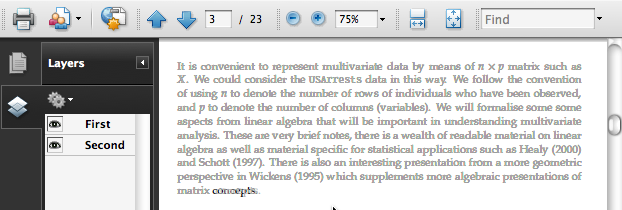
\includegraphics[width=\linewidth]{ar1}

\medskip\noindent
You can see |Layers| icon, clicking on the icon will show you the
layers.  We have two layers in this example, namely, |First| and
|Second| which are also the default.  These labels can be changed with
|\FirstDoc| and |\SecondDoc| commands respectively. 

\subsubsection*{First Document}
\noindent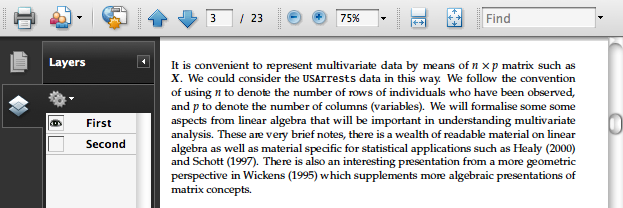
\includegraphics[width=\linewidth]{ar2.png}

\medskip\noindent The above figure shows the first document alone. You
might note that icon for second layer is not visible now.

\subsubsection*{Second Document}
\noindent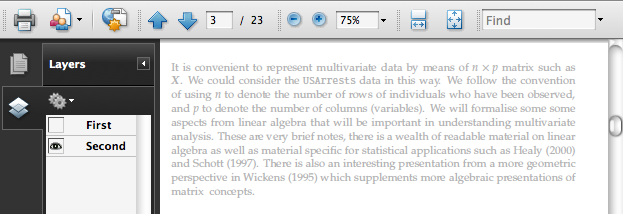
\includegraphics[width=\linewidth]{ar3.png}

\medskip\noindent The second document is generated with 30\% gray
instead of black to facilitate easy indication of locations with
differences. Also, note that icon for first layer is invisible since
the second layer alone is mode visible here.

\section{Examples}

You might take a look at Clip \ref{clip1} which has a paragraph from
the composite document. The last word of the paragraph has a
mismatch. 

\src{A paragraph from composite document.}
\includeclip{3}{104 419 508 556}{ltest.pdf}

Now let us take a look at the last two lines of the above para from
the first document:

\src{Last two lines from first document.}
\includeclip{3}{104 380 508 408}{file1.pdf}

Here is the same location of the second document:

\src{Last two lines from second document.}
\includeclip{3}{104 380 508 408}{file2.pdf}

\noindent The difference is a space added before the last word
`concepts'. If you look at Clip \ref{clip1} now, you will get to know
the difference quickly.

Further differences can be observed in pages 9 and 17 of the included
document, |ltest.pdf|.

\section{Limitations}
Following limitations apply:
\begin{enumerate}
\item Documents with enormous changes cannot be comapared.
\item Documents with opaque backgrounds cannot be compared.
\item Tables and figures with background will not provide any
  meaningful information even if there are differences.
\item This is not a character by character or word by word diff
  program, instead it depends largely on your eyes very much.
\item |pdfpagediff| will work only with \pdftex and will not work with
  any other \tex compilers.

\end{enumerate}

\section{Acknowledgements}

The test document is a chapter namely, |matrices.tex| from a freely
available textbook, \emph{Matrix Overview} by Paul Hewson, at:
\url{http://knowledgeforge.net/opentextbook/svn/multivariatestatistics/}.
Permission to use this chapter to demonstrate the features of
|pdfpagediff| is gratefully acknowledged.

\section{Download}

The package can be downloaded from
\url{http://www.ctan.org/pkg/pdfpagediff}.  Bug
reports, feature requests and suggestions can be posted at
\url{http://www.cvr.cc/pdfpagediff/}.  The author can be contacted at 
\url{<cvr@cvr.cc>}.

\end{document}
